\documentclass[a4paper,fleqn]{cas-sc}
\usepackage{booktabs}
\usepackage{graphicx}
\usepackage{hyperref}
\usepackage{array}
\usepackage{float}
\usepackage{placeins}
\begin{document}
\RenewDocumentCommand \printorcid { } { }
\shorttitle{Controlled Exact N-Queens Benchmark}
\shortauthors{}
\title[mode=title]{Controlled SAT, CP, and MIP Experiments for the N-Queens Problem}
\begin{abstract}
We study the ordinary N-Queens feasibility problem using four CNF at-most-one
encodings---Pairwise, Sequential Counter, Binary, and Commander---with the
Glucose3 and CaDiCaL backends. The primary controlled benchmark contains 300
records with five repetitions per executed cell and a 10-second timeout. SAT
backends cover $N\in\{4,8,16,32,64\}$; the DPLL fallback covers $N=4,8$ and
CPLEX MIP covers $N=4,8$ because of the Community Edition model-size limit.
CP Optimizer and Gurobi cover all five sizes. The primary data contain 250 SAT
and 50 FEASIBLE outcomes, and all 300 returned placements pass an independent
validator. A separate CP-SAT run contains 25 OPTIMAL trials, five each at
$N=4,8,16,32,64$, with all returned placements validated. FEASIBLE is kept
distinct from OPTIMAL. Results support
within-family comparisons, but not an unqualified ranking across different
formulations. Peak memory, Product encoding, and scalability to $N=1331$ were
not measured.
\end{abstract}
\begin{keywords}
N-Queens \sep SAT encodings \sep constraint programming \sep integer
programming \sep CP-SAT \sep PySAT
\end{keywords}
\maketitle

\section{Introduction}
The N-Queens problem asks for a placement of $N$ queens on an $N\times N$
board such that no two queens share a row, column, or diagonal. This work
considers the ordinary feasibility problem rather than an optimization
objective. The assignment requires a PySAT-based SAT solver and comparison
with exact ILP/CP approaches, including CPLEX CP, CPLEX MIP, Gurobi, and
CP-SAT where the environment permits. This report presents the verified
project experiments and does not claim to reproduce external experiments.

The experimental questions are narrower than those of the reference study.
We ask how AMO encoding affects runtime when backend and size are fixed, whether
that behavior changes between Glucose3 and CaDiCaL, and how the SAT results
relate descriptively to binary-cell MIP, integer-column CP, and CP-SAT models.
These questions motivate the separation of SAT and model-family results.

\section{Problem formulations}
\subsection{SAT formulation}
Let $x_{r,c}$ be true when row $r$ contains a queen in column $c$. Each row
and column has an exactly-one constraint, represented by an at-least-one clause
and an at-most-one (AMO) encoding. Diagonal conflicts are represented by
binary clauses $\lnot x_{r,c}\lor\lnot x_{r',c'}$ for attacking cells. The
implemented AMO encodings are Pairwise (Binomial), Sequential Counter
\cite{sinz}, Binary, and Commander. PySAT dispatches Glucose3 and CaDiCaL;
the internal DPLL implementation is reported separately and is not treated as
a CDCL backend. Recursive 2-Product is not implemented and is not included.

More formally, for $r,c\in\{0,\ldots,N-1\}$, the cell variables satisfy
\begin{equation}
\sum_{c=0}^{N-1} x_{r,c}=1 \quad\text{and}\quad
\sum_{r=0}^{N-1} x_{r,c}=1.
\end{equation}
For every pair of attacking cells, the SAT model contains the corresponding
binary conflict clause. The four implemented AMO encodings differ only in how
the exactly-one constraints are expanded into CNF; diagonal conflicts remain
explicit. This distinction is important when interpreting the clause and
variable counts in the SAT tables.

Pairwise encoding adds a conflict clause for every pair in an AMO group. It
uses no auxiliary variables, but its clause count grows quadratically in the
group size. Sequential Counter introduces a chain of auxiliary variables and
linear-size AMO structure. Binary encoding represents the selected position
with auxiliary bits, trading a compact representation for more indirect
propagation. Commander encoding partitions inputs into local groups and links
them through commander variables. These structural differences explain why
the report measures both CNF size and runtime rather than assuming that the
smallest CNF is always fastest. Recursive 2-Product is outside the implemented
scope.

\subsection{CP and MIP formulations}
The CPLEX MIP and Gurobi adapters use binary cell variables with exact row and
column constraints and diagonal conflict inequalities. CPLEX CP Optimizer uses
one integer column variable per row, an all-different column constraint, and
pairwise diagonal constraints. The OR-Tools CP-SAT adapter uses integer column
variables and all-different constraints for columns and diagonals. Its separate
benchmark was executed with OR-Tools 9.15.6755 in an isolated Python 3.11.9
environment. CP-SAT is reported as a constraint-model family, not as a fourth
SAT encoding.

In the integer-column formulation, $q_r\in\{0,\ldots,N-1\}$ denotes the
column selected in row $r$. The CP models enforce distinct values of $q_r$,
$q_r+r$, and $q_r-r$ (or equivalent pairwise diagonal restrictions). The MIP
models instead use the binary cell variables above. Thus the model-size fields
for CP-SAT are not SAT clause counts; unavailable constraint counts remain
explicitly marked as null in its artifact.

\section{Experimental protocol}
The primary data are stored in the new namespace \texttt{results/p1/}. Each
family has JSON, CSV, and summary artifacts with a run identifier. Glucose3
and CaDiCaL use all four SAT encodings at $N=4,8,16,32,64$; each cell has five
trials. DPLL uses all four encodings at $N=4,8$. CPLEX MIP uses its binary
cell model at $N=4,8$. CP Optimizer and Gurobi use their models at all five
sizes. The timeout is 10 seconds per solver call.

The P1 run uses five repetitions for each executed cell. The separate CP-SAT
run also uses five repetitions for each tested size, but has its own run
identifier and output namespace. Repetition statistics are descriptive: they
show startup effects and run-to-run variation, but do not model hardware-level
uncertainty.

The normalized statuses are SAT, UNSAT, FEASIBLE, OPTIMAL, TIMEOUT, ERROR,
and LICENSE\_LIMIT. A returned placement is accepted only when
\texttt{nqueens.model.validate\_solution} returns true. An UNSAT result does
not contain a placement and is not treated as an invalid SAT result.

For SAT, construction time is CNF encoding time and solver time is the timed
backend interval after construction. For CP/MIP/Gurobi, build time covers
adapter/model construction and solver time covers the solver API call. Total
time is the outer elapsed time around adapter dispatch. These intervals are
reported separately but are not assumed identical across paradigms. SAT
variables/clauses use \texttt{sat\_nvars}/\texttt{sat\_nclauses}; model
variables/constraints use \texttt{model\_nvars}/\texttt{model\_nconstraints}.
Peak RSS was not measured. The recorded environment is Python 3.11.9 on
64-bit Windows 10 build 26200; metadata reports PySAT 1.9.dev15, CPLEX
22.2.0.0, and Gurobi 13.0.3. The earlier P1 environment lacked OR-Tools;
the separate CP-SAT run used OR-Tools 9.15.6755 in its isolated environment.

\section{Correctness and benchmark coverage}
The six complete P1 families contain 300 records: 250 SAT and 50 FEASIBLE.
There are no OPTIMAL records in the primary data. All 300 returned solutions
have \texttt{solution\_valid=true}. The performance sizes are all satisfiable
N-Queens instances, so this matrix does not measure UNSAT runtime scaling.
UNSAT correctness is covered separately by the backend smoke test at $N=3$;
the smoke test also checks SAT at $N=4$.

The DPLL history is kept separate. The initial \texttt{dpll.json} contains 15
ERROR records caused by an early runner configuration defect. The partial
\texttt{dpll\_v2.json} contains 40 SAT records and four TIMEOUT records from
an interrupted $N=16$ attempt. The complete DPLL family used for analysis is
only \texttt{dpll\_final.json}, with 40 records at $N=4,8$.

CPLEX MIP is absent above $N=8$ because the Community Edition limit was
observed at $N=16$ in earlier artifacts. This is an environment/license
limitation, not evidence that the MIP formulation is UNSAT or incapable at
that size.

The separate CP-SAT performance artifact contains 25 records: five OPTIMAL
trials at each of $N=4,8,16,32,64$. These records are not added to the 300
record P1 total because they were collected in a separate run and namespace.

The correctness and performance matrices answer different questions. The
correctness checks include UNSAT cases such as $N=2$ and $N=3$, where no valid
placement exists. The performance matrices use satisfiable sizes so that their
runtime curves describe finding a witness rather than mixing infeasibility
proof with witness construction.

\begin{table}[H]
\centering
\caption{Primary P1 record and status counts.}
\label{tab:coverage}
\begin{tabular}{lrrrrrr}
\toprule
Family & Records & SAT & FEASIBLE & OPTIMAL & TIMEOUT & Valid\\
\midrule
Glucose3 & 100 & 100 & 0 & 0 & 0 & 100\\
CaDiCaL & 100 & 100 & 0 & 0 & 0 & 100\\
DPLL fallback & 40 & 40 & 0 & 0 & 0 & 40\\
CPLEX MIP & 10 & 10 & 0 & 0 & 0 & 10\\
CPLEX CP Optimizer & 25 & 0 & 25 & 0 & 0 & 25\\
Gurobi & 25 & 0 & 25 & 0 & 0 & 25\\
\midrule
Total & 300 & 250 & 50 & 0 & 0 & 300\\
\bottomrule
\end{tabular}
\end{table}

\section{SAT encoding and backend results}
Table~\ref{tab:sat-runtime} gives median total times in seconds over five
completed trials. Comparisons across encodings are made within one backend.

\begin{table}[H]
\centering
\caption{Median total runtime for SAT families; five trials per cell.}
\label{tab:sat-runtime}
\scriptsize
\begin{tabular}{llrrrrr}
\toprule
Backend & Encoding & $N=4$ & $N=8$ & $N=16$ & $N=32$ & $N=64$\\
\midrule
Glucose3 & Pairwise & 0.000473 & 0.001101 & 0.023736 & 0.039814 & 0.376201\\
Glucose3 & Sequential & 0.000485 & 0.001152 & 0.003764 & 0.024729 & 0.140699\\
Glucose3 & Binary & 0.000478 & 0.002096 & 0.003832 & 0.022807 & 0.207304\\
Glucose3 & Commander & 0.000530 & 0.002235 & 0.004662 & 0.021832 & 0.142131\\
CaDiCaL & Pairwise & 0.001069 & 0.001711 & 0.024290 & 0.087844 & 0.890577\\
CaDiCaL & Sequential & 0.001169 & 0.002496 & 0.004889 & 0.180281 & 0.471191\\
CaDiCaL & Binary & 0.001086 & 0.002323 & 0.012405 & 0.119226 & 0.796737\\
CaDiCaL & Commander & 0.001053 & 0.002135 & 0.012587 & 0.034323 & 0.455395\\
\bottomrule
\end{tabular}
\end{table}

Within the observed range, encoding and backend interact. Sequential has the
lowest Glucose3 median at $N=64$ among the four encodings, while Commander has
the lowest CaDiCaL median at $N=32$ and $N=64$ among the displayed values.
These are configuration-specific observations, not a universal ranking.

At $N=64$, Sequential is the fastest Glucose3 configuration in the displayed
table at 0.140699 s, while Pairwise is 0.376201 s. For CaDiCaL at the same
size, Commander is fastest at 0.455395 s and Pairwise is 0.890577 s. The
direction is therefore consistent for these two endpoint comparisons, but it
does not imply a globally best encoding: at $N=4$ the four medians are all
within a narrow range, and the ordering changes at smaller sizes. The backend
effect is also encoding-dependent. For example, Pairwise at $N=64$ is slower
with CaDiCaL than with Glucose3, whereas the relevant comparison for another
encoding can have a different gap. These observations support an interaction
between encoding structure and solver heuristics, not a claim that one backend
dominates for every formulation.

The construction and solver intervals provide a second perspective. SAT
construction time is the CNF-generation interval, while the displayed runtime
table uses total time. Thus a runtime difference should not be attributed to
search alone unless the solver-time field is examined as well. The available
plots and group statistics preserve this distinction; no peak-memory or
propagation-depth conclusion is drawn because those metrics were not measured.

\begin{figure}[H]
\centering
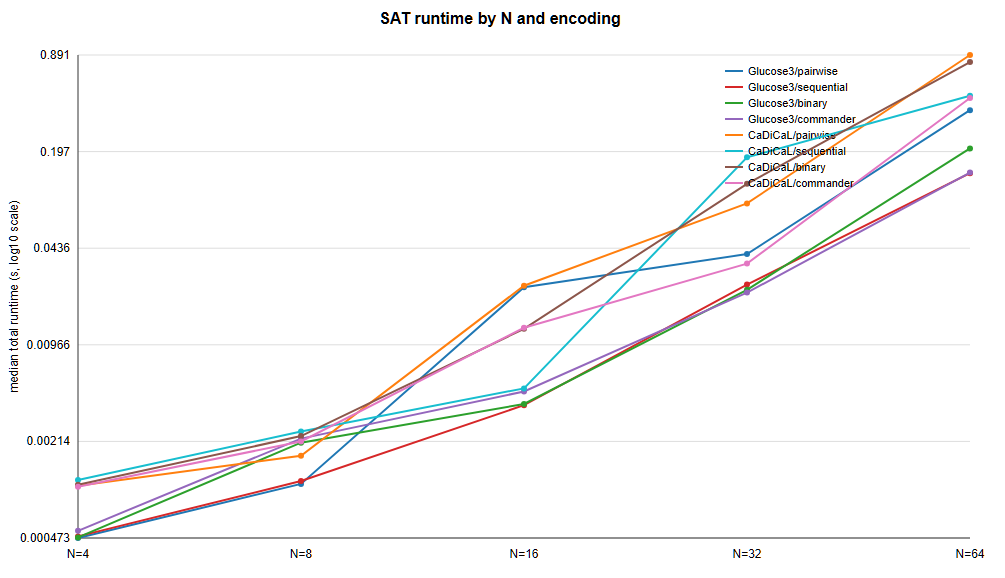
\includegraphics[width=0.76\linewidth]{build/generated/sat_runtime_by_n.png}
\caption{Median SAT runtime by board size, backend, and encoding; logarithmic vertical scale.}
\label{fig:sat-runtime}
\end{figure}
\begin{figure}[H]
\centering
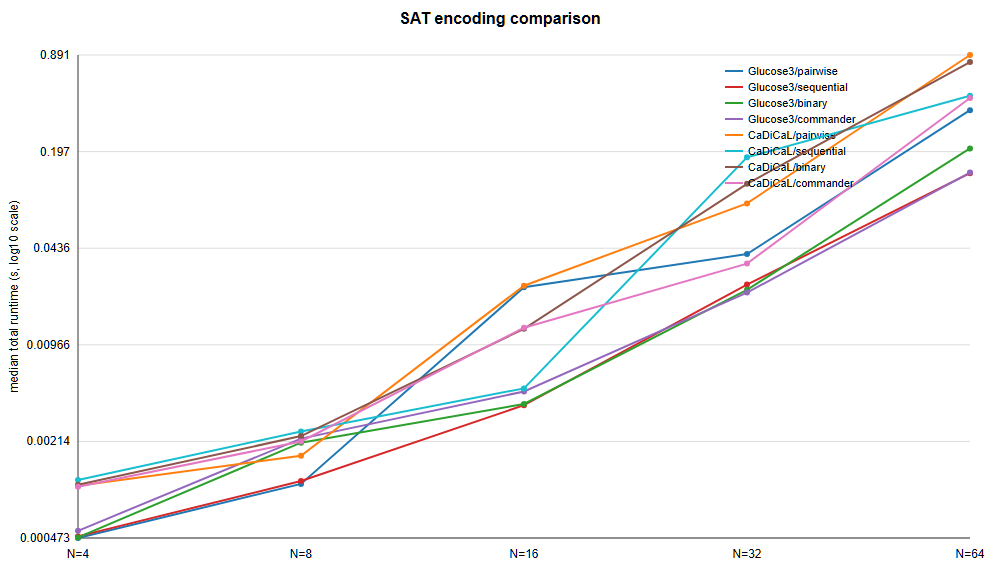
\includegraphics[width=0.76\linewidth]{build/generated/sat_encoding_median_runtime.png}
\caption{Median runtime comparison among the four SAT encodings.}
\label{fig:sat-encoding}
\end{figure}
\begin{figure}[!htbp]
\centering
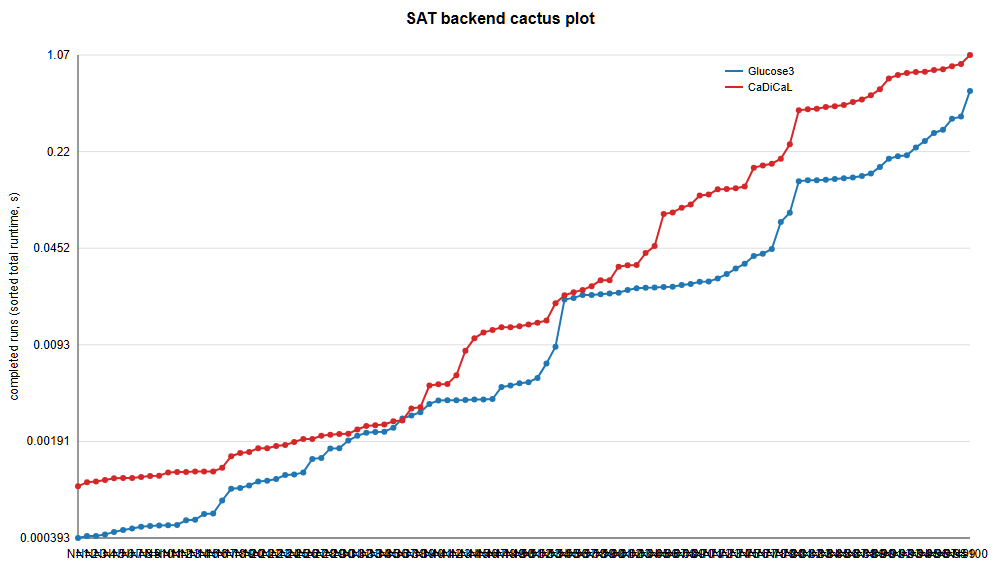
\includegraphics[width=0.76\linewidth]{build/generated/sat_cactus.png}
\caption{Cactus plot of completed SAT records; no timeout is assigned a finite runtime.}
\label{fig:sat-cactus}
\end{figure}

\section{CP and MIP model-family results}
Table~\ref{tab:model-runtime} reports model-family medians separately. CP
Optimizer and Gurobi return FEASIBLE placements; these are not relabeled
OPTIMAL. CPLEX MIP has no primary observations at $N=16$ or above.

\begin{table}[H]
\centering
\caption{Median total runtime in seconds for model-family formulations. CP-SAT
values come from a separate 25-trial artifact and are not part of the 300
record P1 total.}
\label{tab:model-runtime}
\begin{tabular}{lrrrrr}
\toprule
Family & $N=4$ & $N=8$ & $N=16$ & $N=32$ & $N=64$\\
\midrule
CPLEX MIP & 0.025620 & 0.043730 & -- & -- & --\\
CPLEX CP Optimizer & 0.034450 & 0.032524 & 0.039662 & 0.059330 & 0.261713\\
Gurobi & 0.002051 & 0.003109 & 0.033490 & 0.243846 & 2.082438\\
CP-SAT & 0.072137 & 0.119335 & 0.189959 & 0.376305 & 1.630790\\
\bottomrule
\end{tabular}
\end{table}

These values are descriptive within each formulation and environment. The
different formulations and timing intervals do not justify one cross-paradigm
ranking.

The separate CP-SAT run has median total times of 0.072137, 0.119335,
0.189959, 0.376305, and 1.630790 seconds for $N=4,8,16,32,64$, respectively.
All 25 statuses are OPTIMAL and all 25 returned placements pass independent
validation. The N=4 mean is 0.801006 seconds versus a median of 0.072137
seconds because the first trial took 3.712484 seconds; this trial is retained.
CP-SAT model-constraint count was not measured and is left unavailable.

The model-family table should be read as four separate descriptive series.
CPLEX MIP has observations only at $N=4$ and $N=8$, so its missing larger
values are license-limited omissions rather than timeouts or UNSAT results.
CP Optimizer returns FEASIBLE placements throughout its P1 range, while the
separate CP-SAT run returns OPTIMAL statuses; these status labels are not
interchangeable. Gurobi is also recorded as FEASIBLE in P1. Consequently, the
lower runtime of one row cannot be interpreted as a proof of superiority when
the formulations, status guarantees, and run namespaces differ.

Within CP-SAT itself, the median total increases from 0.072137 s at $N=4$ to
1.630790 s at $N=64$, with solver time dominating the recorded total from
$N=8$ onward. The mean at $N=4$ is 0.801006 s while the median is 0.072137 s
because the first trial took 3.712484 s. That trial is retained because it is
part of the raw five-trial experiment. This is evidence about the measured
CP-SAT configuration through $N=64$, not evidence of scalability to $N=1331$.

\begin{figure}[H]
\centering
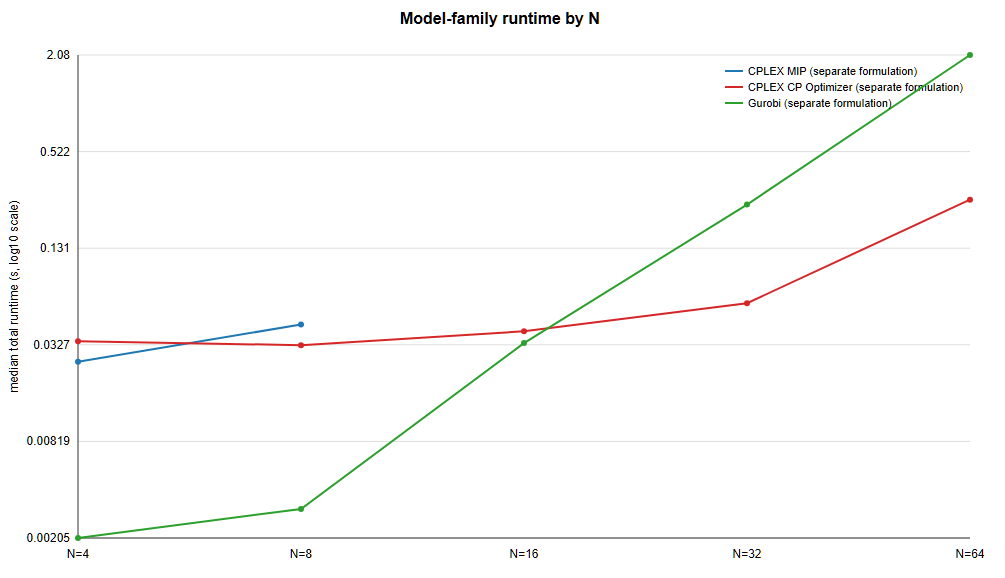
\includegraphics[width=0.76\linewidth]{build/generated/model_family_runtime.png}
\caption{Runtime curves for the P1 model families; CP-SAT is reported in the
separate table because its artifact uses a separate run and formulation.}
\label{fig:model-runtime}
\end{figure}
\begin{figure}[H]
\centering
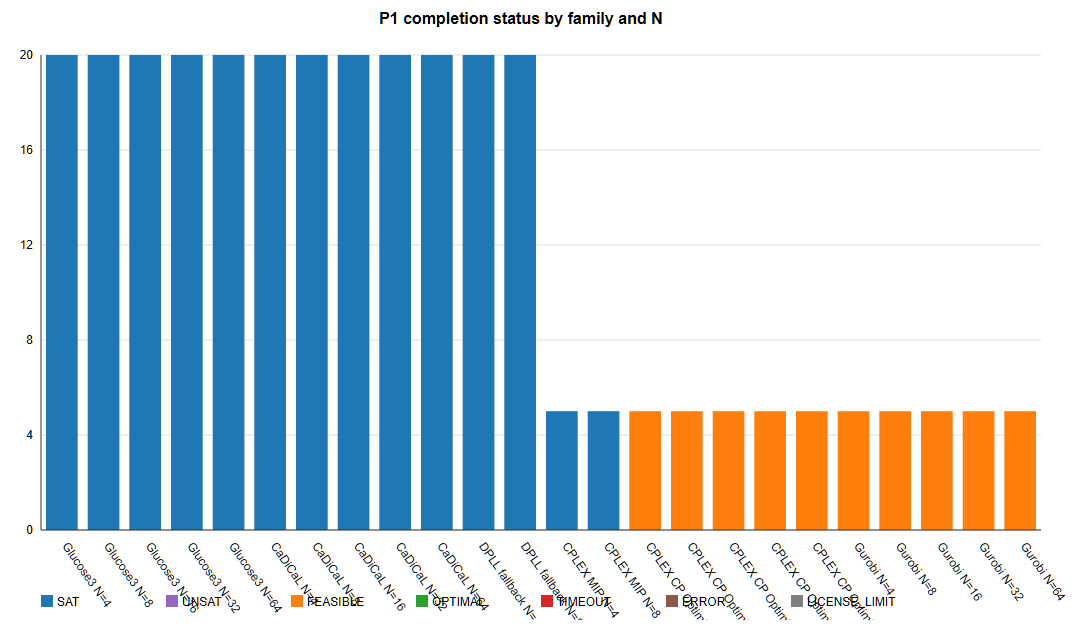
\includegraphics[width=0.76\linewidth]{build/generated/completion_status_by_n.png}
\caption{Status counts by family and board size for complete P1 families.}
\label{fig:completion}
\end{figure}
\FloatBarrier

\section{Discussion and limitations}
The P1/P2 data support validated within-family comparisons through $N=64$.
They do not establish scalability to $N=1331$, because no such run exists.
The DPLL partial run provides evidence of repeated timeouts at $N=16$, but it
is not a complete five-trial cell and is not combined with final DPLL results.

The performance matrix contains only satisfiable sizes. UNSAT is therefore a
correctness outcome, not a measured large-size performance category. The report
does not assign finite runtimes to TIMEOUT or ERROR. The final P1 families
happen to have no TIMEOUT or ERROR records, while the separate DPLL artifacts
preserve four TIMEOUT and 15 ERROR records.

CP-SAT was benchmarked separately after OR-Tools became available in an
isolated environment. Its 25 trials are not directly ranked against the P1
families because the run has a separate scope and constraint formulation.
Product encoding is not implemented. Peak resident memory, CPU utilization,
and process-level resource monitoring were not measured. The reference paper's
N=1331, Product, memory, and 252-run results are reference results, not project
results.

Historical artifacts remain separate from P1. The earlier comparison and
medium matrices are not merged into the 300 primary records because they use
different scopes and schemas. P1/P2 tables and plots are generated from
\texttt{results/p1/} and \texttt{results/p2\_p3/}; group statistics are stored
in \texttt{p1\_group\_statistics.csv} and \texttt{p1\_group\_statistics.json}.

\section{Conclusion and future work}
This study provides a controlled comparison of four SAT encodings with two
PySAT backends, together with separate DPLL, CP, and MIP model families. All
300 returned primary placements passed independent validation. The results
show that encoding and backend interact within the tested range, while CP/MIP
results must be interpreted within their own formulations.

The data do not establish a universal winner, equivalence of OPTIMAL and
FEASIBLE results, scalability to $N=1331$, or memory efficiency. The separate
CP-SAT run demonstrates successful OPTIMAL results through $N=64$ under its
own constraint formulation, but does not establish cross-paradigm superiority.
Larger-size experiments are appropriate only if the assignment requires sizes
beyond $N=64$ or a scalability claim is desired. Product encoding and memory
monitoring remain optional research extensions.

\section*{Data Availability}
The source code and benchmark artifacts are maintained in the project
repository: \url{https://github.com/DunnTapCodee/N-Queens-Solver}. Primary
records are in \texttt{results/p1/}; derived statistics and plots are in
\texttt{results/p2\_p3/}. The separate CP-SAT records are in
\texttt{results/cp\_sat/}. The analysis can be regenerated with
\texttt{python scripts/analyze\_p1.py}. Historical files under
\texttt{results/raw/} are preserved separately.

\begin{thebibliography}{00}
\bibitem{sinz} C. Sinz, ``Towards an optimal CNF encoding of Boolean
cardinality constraints,'' in \emph{Principles and Practice of Constraint
Programming}, 2005.
\bibitem{pysat} PySAT developers, ``SAT solvers' API (pysat.solvers),'' official
documentation, \url{https://pysathq.github.io/docs/html/api/solvers.html}.
\end{thebibliography}
\end{document}
